\section{Demonstration}

\subsection{Spatial Queries}

In Geo-Store, we implemented three basic spatial filters as
building blocks for constructing complex spatial queries.

\underline{\textbf{Window Filter}} \\
A window filter describes a binding of a query variable in a
SPARQL query to a specified rectangular region in a 2-dimensional
space.

\begin{verbatim}
SELECT ?name ?location WHERE{
    ?e <name> ?name.
    ?e <coordinates> ?location.
    within(?location, 32.5955, -85.4909, 32.6122,
           -85.4739)
}
\end{verbatim}
%\caption{\small Skyline SQL Clause.
%\label{fig:skyline_sql}}

\underline{\textbf{Range Filter}} \\
A range filter imposes a binding of a query variable in a SPARQL
query to a circular region in a 2-dimensional space, given a
center point and a radius.

\begin{verbatim}
SELECT ?name ?location WHERE{
    ?e <name> ?name.
    ?e <coordinates> ?location.
    within(?location, 32.597178, -85.463086, 1500)
}
\end{verbatim}

\underline{\textbf{Nearby Filter}} \\
A nearby filter can be used to issue a \emph{k}-NN query, given
the location of a query point and the \emph{k} value.

\begin{verbatim}
SELECT ?name ?location WHERE{
    ?e <name> ?name.
    ?e <coordinates> ?location.
    nearby(?location, 32.607985, -85.481439, 3)
}
\end{verbatim}

\subsection{Query Builder}

Figure~\ref{fig:geostore_web} shows the GUI of the query builder.
The GUI consists of two parts. The top part is the query editor
that allows the user to manually enter a SPARQL query with
aforementioned spatial query filters. The bottom part is the
interface that prompts the user to provide the corresponding query
parameters so that spatial filters can be generated automatically
and inserted into a standard SPARQL query incrementally. To
evaluate a SPARQL query with spatial constraints/patterns, the
spatial constraints are first dealt with by our spatial query
analyzer while the non-spatial constraints are submitted to the
underlying triple store
RDF-3X~\cite{DBLP:journals/vldb/NeumannW10} for execution.

\begin{figure}[t]
\centering
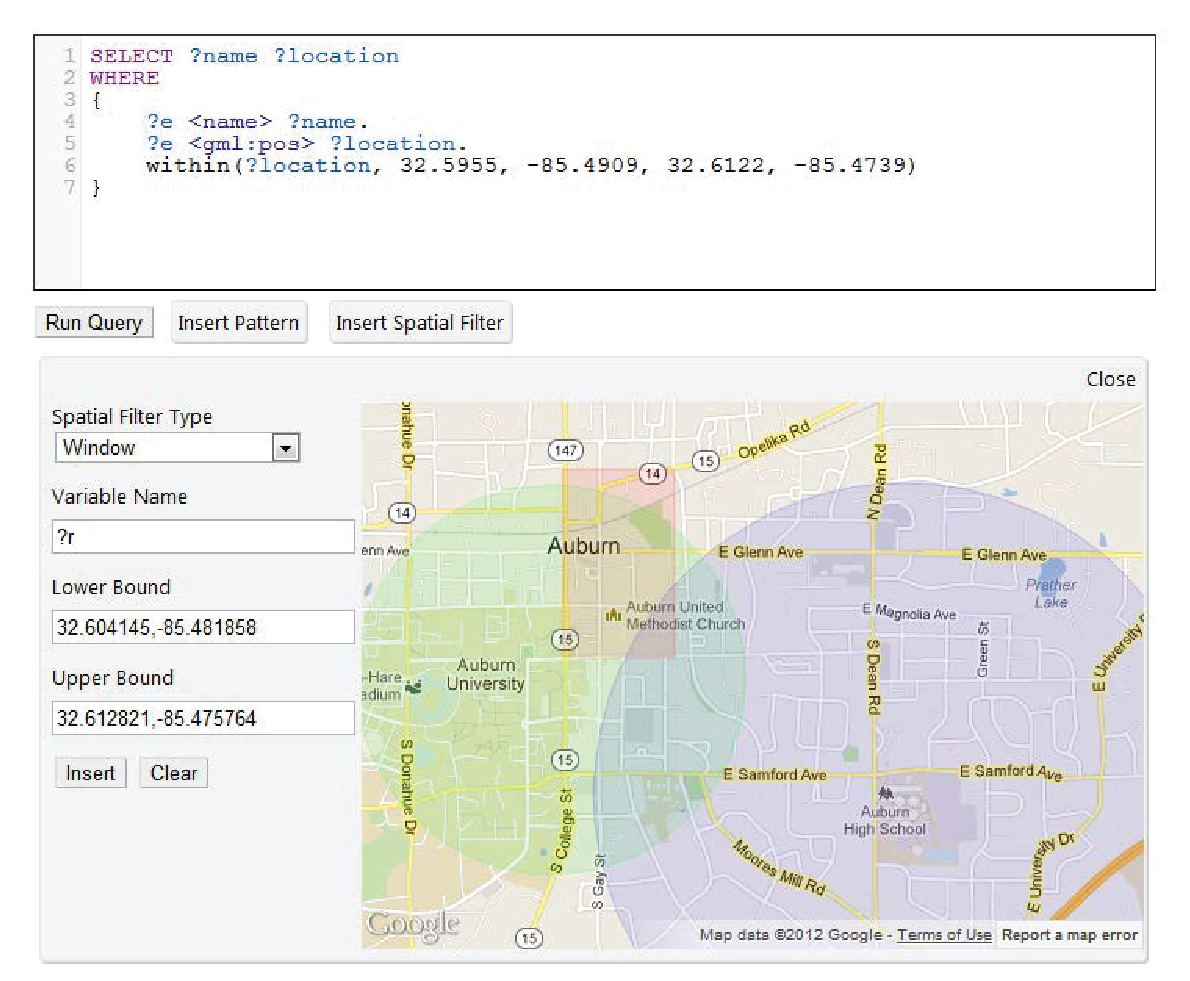
\includegraphics[width=3.3in]{images/geostore_web.eps}
\caption{Query Builder GUI of Geo-Store}\label{fig:geostore_web}
\end{figure}
